\documentclass[a4paper,11pt,epsf]{article}

\usepackage[latin1]{inputenc}
\usepackage[spanish]{babel}

\usepackage{graphicx}
\usepackage{epsfig}

\usepackage{fancyvrb}

\renewcommand{\FancyVerbFormatLine}[1]{\parbox[t]{\textwidth}{\indent #1}}

\newcommand{\includescript}[1]{\VerbatimInput[showtabs=1,obeytabs=1,tabsize=8,frame=single,label=\fbox{\bf \large #1},gobble=0, numbers=left, fontsize=\footnotesize]{#1}}

\newcommand{\includescriptnonumbers}[1]{\VerbatimInput[showtabs=1,obeytabs=1,tabsize=8,frame=single,label=\fbox{\bf \large #1},gobble=0, fontsize=\footnotesize]{#1}}


\usepackage{fancyhdr}
\oddsidemargin 	0pt
\evensidemargin	0pt
\textwidth 	440pt
\textheight 	660pt
\headheight 	10pt
\topmargin	0pt
\headsep 	20pt
\pagestyle{fancy}
\rhead{ITBA}
\lhead{Sistemas Operativos}
\renewcommand{\headrulewidth}{0.5 pt}
\renewcommand{\footrulewidth}{0.5 pt}
\renewcommand{\textfraction}{0.15}
\renewcommand{\topfraction}{0.85}
\renewcommand{\bottomfraction}{0.65}
\renewcommand{\floatpagefraction}{0.60}
\setlength{\parskip}{6pt}

\title{
{\large \bfseries Trabajo Pr\'actico Especial de Sistemas Operativos}
\\
\vspace{24pt}
\textbf{FLEDS}
}

\author{Abramowicz, Pablo Federico \\ 
Go\~ni, Juan Ignacio \\ 
Pan, Matias Santiago\\
$\phantom{1}$ \\ 
\textsc{Instituto Tecnol\'ogico de Buenos Aires} }

\date{}


\begin{document}
\maketitle

\newpage

\tableofcontents

\newpage

\begin{abstract}
Este informe t\'ecnico presenta la implementaci\'on de un dispositido de leds y su respectivo controlador para el sistema operativo Minix $2.0.0$. Se incluye las descripciones t\'ecnicas del dispositivo y las modificaciones realizadas a los c\'odigos fuente para la vinculaci\'on con el controlador.\\ 
\textbf{Keywords:} \textit{fleds, driver, hardware, interrupciones de hardware, IRQ, handler, serial.} 
\end{abstract}

\section{Introducci\'on}

Este proyecto surgi\'o debido a la consigna de la c\'atedra de agregarle alguna funcionalidad a Minix $2.0.0$. El primer proyecto que se nos ocurri\'o fue vincular Minix con GPS mediante el puerto serial, pero el hecho de que Minix no contase con un X imposibilitaba visualizar el mapa de forma coherente, agregando que la complejidad del dispositivo de GPS era parsear la telemetr\'ia entregaba. Luego de discutir, surgi\'o la idea de armar un \emph{cartel del leds}, de ahora en m\'as \textbf{Fleds}, y a continuaci\'on se pasa a detallar los detalles del mismo.

\section{Implementaci\'on}
En principio se pens\'o en realizar la comunicaci\'on entre Minix y el \textbf{Fleds} compuesta por 2 capas: una donde el usuario pueda comunicarse y mandarle los comandos, y otra donde el driver se comunique con el fleds por medio del puerto serial. La misma ser\'ia:

\textbf{Usuario $\rightarrow$ driver fleds $\rightarrow$ driver serial $\rightarrow$ fleds hardware}

Luego de investigar y revisar el controlador provisto por minix del serial (\verb./usr/src/kernel/RS232.c) se lleg\'o a la concluci\'on de que era pr\'acticamente inutilizable debido a la estrecha vinculaci\'on del mismo con la terminal (\verb./usr/src/kernel/tty.c), a lo cual se procedi\'o a realizar un \'unico controlador que haga de ambos.

A su vez, se pens\'o en dejar la l\'ogica del controlador del lado del usuario por un tema de espacio en la ROM del Hardware, pero satisfactoriamente se pudo incluir ciertas l\'ogicas dentro del Hardware. 

Tambi\'en se gener\'o una librer\'ia de animaciones para una f\'acil utilizaci\'on del mismo. 

\section{Hardware}
\textbf{Fleds} consta de 128 leds rgb, con la capacidad de encenderse con los 3 colores primarios luz, rojo, azul y verde, independientemente.  Consta de 16 columnas por 8 filas. Se utiliz\'o un decodificador para la selecci\'on de la columna, 3 latches para el dibujado de los colores y un microcontrolador para el refresco de la pantalla.  En la figura \ref{design} se muestra el diagrama del circuito.

\begin{figure}
\centering
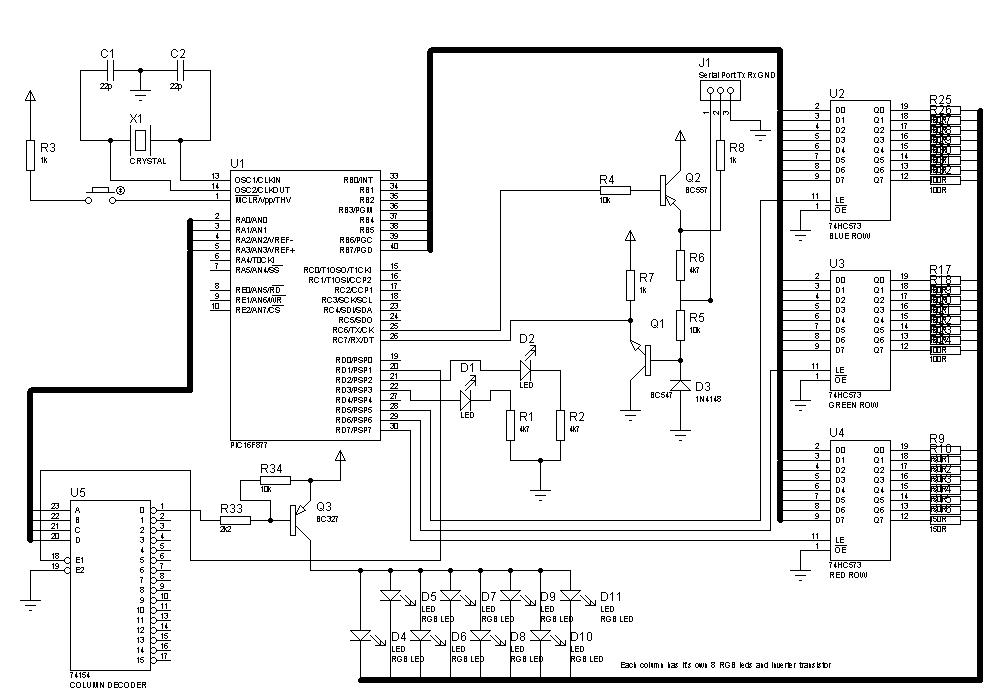
\includegraphics[scale =0.5]{design.png}
\caption{Dise\~no del circuito el\'ectrico de FLEDS}\label{design}
\end{figure}

\subsection{Principio de funcionamiento}
En el microcontrolador tiene cargado el firmware, el cual se encarga de mantener la comunicaci\'on con el driver de Minix v\'ia puerto serial. 
Cuando recibe un byte, se genera una interrupci\'on, la cual analiza seg\'un el protocolo el comando recibido y lo ejecuta. 
En estado normal, mantiene el refresco de la pantalla. Primero, le indica al decodificador que debe habilitar la primer columna, luego, se setean en cada latch, la columna del rojo, verde y azul. Se espera un milisegundo, y se proceden a dibujar las siguientes columnas, hasta llegar a la \'ultima, donde vuelve a comenzar el ciclo. El refresco es de 60Hz aproximadamente.

\subsection{Protocolo}
Se enumeran los comandos implementados en el firmware:


\textbf{0x00}: Clear screen. Borra la pantalla \\


\textbf{0x40 al 0x4F}: Set column. Establece la combinaci\'on de colores para la columna del nibble menos significativo (0 a 15). Recibe por par\'ametros los 3 bytes para el rojo, verde y azul, respectivamente. \\


\textbf{0x10 al 0x19}: Scroll. Realiza un scroll en base al valor del nibble menos significativo. 0 para ScrollDownCarry, 1 para ScrollDown, 2 para ScrollUpCarry, 3 para ScrollUp, 4 para ScrollLeftCarry, 5 para ScrollLeft, 6 para ScrollRightCarry, 7 para ScrollRight, 8 para  StartScroll y 9 para StopScroll. \\


\textbf{0x08 al 0x8F}: Set UART speed. Establece la velocidad de la UART en base al nibble menos significativo.  0 para 1200, 1 para  2400, 2 para 4800, 3 para 9600, 4 para 19200, 5 para 38400, 6 para 57600 y 7 para 115200 baudios. \\


\textbf{0x20 al 0x2F}: Set scroll speed. Establece la frecuencia para el scroll.\\


\textbf{0x5A}: Get screen. Transmite por el serial, el contenido actual de la  pantalla, enviando 96 caracteres encerrados entre [ y ], para su mejor lectura. \\

\section{Controlador}
La implementaci\'on del driver del fleds involucr\'o la modificaci\'on de c\'odigos fuentes del kernel de Minix y el agregado de nuevos archivos. Se detalla a continuaci\'on las modificaciones correspondientes con sus respectivas explicaciones. 
\textit{Aclaraci\'on: Los paths que encabezan las siguientes subsecciones son relativos a \emph{\/usr\/}., y representan la locaci\'on del archivo en el file-system.}

\subsection{include/minix/com.h}

Este archivo contiene los n\'umeros de tareas que involucra el kernel, a lo cu\'al se procedi\'o a cambiar el n\'umero de tarea de la \textbf{TTY} como \'ultimo y agregarle la tarea del \textbf{Fleds} para que el kernel la pueda manejar.

\includescript{com-min.h}

\subsection{include/minix/config.h}

En este archivo se definen configuraciones que se van a utilizar. Como se est\'a agregando un nuevo dispositivo, se agrega la definici\'on del \textbf{ENABLE} del mismo.

\includescript{config-min1.h}

Tambi\'en se procedi\'o a deshabilitar el serial utilizado por la TTY poniendo \verb.NR_RS_LINES. en 0.

\includescript{config-min2.h}

\subsection{include/minix/const.h}

El \verb.NR_TASK. contiene la cantidad de tareas que corre inicialmeten el kernel, a lo cual, como se est\'a agregando un controlador y se desea que est\'e activado todo el tiempo, agregamos la tarea

\includescript{const-min.h}

\subsection{src/kernel/table.c}

En principio se tiene que agregar el tama\~no de stack correspondiente al controlador. En \verb.FLEDS_STACK. se define el mismo como un \verb.SMALL_STACK.

\includescript{table-min.c}

Tambi\'en se tiene que agregar el mismo al tama\~no total de stack definido en \verb.TOT_STACK_SPACE..

\includescript{table-min2.c}

El \textbf{struct tasktab tasktab[]} contiene el punto de entrada de las tareas que se ejecutan, a lo cual se debe agregar la tarea del controlador del \textbf{Fleds}. Para agregar una entrada se debe especificar primero la funci\'on encargada de atender los pedidos al controlador, en nuestro caso \verb.fleds_task., luego se define el stack correspondiente de la tarea, en nuestro caso \verb.FLEDS_STACK., y por \'ultimo se define el nombre de la tarea a mostrar.

\includescript{table-min3.c}

Es importante que se agregue en conconrdancia al n\'umero de tarea incluido en \verb./include/minix/com.h. Entonces, como se incluy\'o en segundo lugar, aqu\'i se hace de la misma manera.

\subsection{src/fs/table.c}

La tabla \verb.dmap. determina la vinculaci\'on entre el n\'umero principal y la tarea que recibe el mensaje. En la misma se agreg\'o en una posici\'on libre, la 9, la tarea de Fleds. 

\includescript{fs-table-min.c}


\subsection{src/kernel/fleds.c}

Este archivo contiene realmente el controlador del dispositivo. Contiene una \'unica funci\'on p\'ublica \verb.fleds_task(). que es el proceso controlador y la comunicaci\'on con el mismo se hace mediante las primitivas \verb.open., \verb.close., \verb.read. y \verb.write..
Inicialmente, cuando arranca el controlador inicializa el serial debido que ya no lo hace m\'as la tty. En este proceso se involucra los seteos de la velocidad, paridad, interrupci\'on, buffers internos, etc. Luego la tarea queda esperando a recibir alg\'un mensaje. Una de las complejidades surgidas fue el tema de los direccionamientos que utiliza minix en modo kernel y en modo usuario y el requerimento de copiar los datos entre los distintos segmentos (en el caso de \verb.write. y \verb.read.).

\includescript{fleds.c}

\subsection{src/kernel/fleds.h}

Este archivo contiene la configuraci\'on del Fleds.

\includescript{fleds.h}

\section{Aplicaci\'on}

A modo de utilizaci\'on del Fleds se implement\'o una librer\'ia libFleds.c destinada a facilitarle el uso del mismo al usuario, la misma incluye las siguientes funciones:

\subsection{fledsADT newFleds (int height, int width, char * device)}
Crea una nueva instacia del Fleds.

\subsection{int freeFleds (fledsADT fleds)}
Libera la instancia del Fleds.

\subsection{int loadText (fledsADT fleds, char * text, int x, int y)}
Carga un texto dado en el Fleds dadas las coordenadas x, y.

\subsection{int loadPic (fledsADT fleds, pic\_t pic, int x, int y)}
Carga una imagen dado un pic\_t en las coordenadas dadas.

\subsection{int loadMovie (fledsADT fleds, pic\_t * pic)}
Carga una pel\'icula en un vector de pic\_t.

\subsection{int clear (fledsADT fleds)}
Limpia la pantalla del Fleds.

\subsection{int show (fledsADT fleds)}
Activa la imagen que tiene cargado el Fleds. Prende los leds.

\subsection{int hide (fledsADT fleds)}
Oculta lo que est\'a mostrando el Fleds. Apaga los leds.

\subsection{int animate (fledsADT fleds, animation\_t animation, int iterations, int speed)}
Anima los datos cargados en el Fleds con un tipo de animaci\'on. Existen diferentes tipos de animaci\'on, los cuales son:
\subsubsection{SCROLL\_NONE}
No hace ning\'un tipo de scroll.
\subsubsection{SCROLL\_RIGHT}
Scroll hacia la derecha y borra el contenido.
\subsubsection{SCROLL\_LEFT}
Scroll hacia la izquierda y borra el contenido.
\subsubsection{SCROLL\_UP}
Scroll hacia arriba y borra el contenido.
\subsubsection{SCROLL\_DOWN}
Scroll hacia abajo y borra el contenido.
\subsubsection{SCROLL\_RIGHT\_CARRY}
Scroll hacia la derecha y hace c\'iclico el muestreo. 
\subsubsection{SCROLL\_LEFT\_CARRY}
Scroll hacia la izquierda y hace c\'iclico el muestreo. 
\subsubsection{SCROLL\_UP\_CARRY}
Scroll hacia arriba y hace c\'iclico el muestreo. 
\subsubsection{SCROLL\_DOWN\_CARRY}
Scroll hacia abajo y hace c\'iclico el muestreo. 
\subsubsection{SCROLL\_ROW\_LEFT}
Scrolea fila por fila hacia la izquierda limpiando la pantalla.
\subsubsection{SCROLL\_ROW\_RIGHT}
Scrolea fila por fila hacia la derecha limpiando la pantalla.
\subsubsection{SCROLL\_COLUMN\_DOWN}
Scrolea columna por columna hacia abajo limpiando la pantalla.
\subsubsection{WAVE}
Hace \emph{la ola} con la imagen puesta en el fleds.
\subsubsection{TWINKLE}
Parpadea el contenido de la pantalla.
\subsubsection{LSD}
Tira animaciones re-locas.
\subsubsection{MOVIE}
Anima la pelicula.
\subsubsection{CAMEL}
Genera el efecto camel que tanto se comenta entre los j\'ovenes.
\section{Conclusiones} 
Creemos haber cumplido el objetivo que nos planteamos al comienzo del tpe, desarrollar un dispositivo f\'isico de leds y su respectivo driver para el sistema operativo Minix.\\
Se comprendi\'o la interacci\'on de Minix internamente, el armado de un controlador nuevo y la vinculaci\'on entre s\'i.\\
Finalmente, estamos satisfechos con el resultado obtenido y consideramos \'esta una experiencia muy positiva.

\section{Posibles extensiones} 
Se podr\'ia agregar dentro de lo que es el controlador la posibilidad de cambiarle par\'ametros de conexi\'on con el dispositivo utilizando ioctl. Actualmente est\'a definido pero no se est\'a utilizando. Respecto al dispositivo, agregar m\'as m\'odulos para mostrar im\'agenes con una mayor resoluci\'on o textos m\'as largos.

\begin{thebibliography}{10}

\bibitem{libro1} ``\textit{Sistemas Operativos. Dise\~no e implementaci\'on}'' - Andrew S. Tanenbaum, Albert S. Woodhull
\bibitem{libro2} ``\textit{Intro\_minix.pdf}'' - C\'atedra de Sistemas Operativos
\bibitem{link} ``\textit{Dise\~no de Sistemas Operativos}'' - http://gsd.unex.es/~jdiaz/asig/dso/lab/p8/p8\_v2.pdf
\bibitem{source} ``\textit{Librer\'ias fuentes de Minix}'' - /usr/ dentro de minix.
\end{thebibliography}

\end{document}

